\documentclass{article}
\usepackage[utf8]{inputenc}
\usepackage{graphicx}

\title{TC genesis tabs and figs}
\author{slnazhangtao }
\date{September 2018}

\begin{document}

\maketitle

\section{Tables}

 \begin{table} % T1
 \caption{List of environmental factors for TC genesis}
 \centering
 \begin{tabular}{l l l}
 \hline
 Variable &  Abbreviation & Dataset source \\
 \hline
 Longitude                                  & lon           & MCS dataset\\
 Latitude                                   & lat           & MCS dataset\\
 Month                                      & mon           & MCS dataset\\
 Genesis potential index                    & GPI           & ERA-Interim\\
 850hPa vorticity                           & Vort850       & ERA-Interim  \\
 600hPa relative humidity                   & Q600          & ERA-Interim  \\
 Vertical wind shear from 850hPa to 200hPa  & wind\_shear   & ERA-Interim   \\
 TC Potential intensity                     & TC\_PI        & ERA-Interim\\
 MCS area coverage                          & MCS\_size     & MCS dataset\\
 Average BT of all pixels with a MCS        & MCS\_avgBT    & MCS dataset   \\
 Lowest BT of all pixels with a MCS         & MCS\_minBT    & MCS dataset  \\
 Propagation speed of a MCS                 & MCS\_speed    & MCS dataset \\
 Movement direction of a MCS                & MCS\_direct   & MCS dataset\\ 
\hline
\end{tabular}
\end{table}

\begin{table} [h]%T2
\centering
\caption{Classifiers used in this study}
\label{my-label}
\begin{tabular}{lll}
\hline
category                & Classifier                        & Abbreviation \\ \hline
{Linear}                & Logistic Regression               & Logist       \\
                        & Naive Bayes                       & NB           \\ \hline
{Nonlinear}             & Decision Tree                     & DTree        \\
                        & K  Nearest  Neighbours            & KNN          \\
                        & Multilayer Perceptron             & MLP          \\
                        & Quadratic Discriminant Analysis   & QDA          \\
                        & Support Vector Machines           & SVM          \\ \hline
{Nonlinear ensemble}    & Adaboost                          & ADA          \\
                        & Random Forests                    & RFs          \\
\hline
\end{tabular}
\end{table}

\begin{table}[h] %T3
 \caption{The confusion matrix/contingency table showing the four possible outcomes for a 2-class 
 developing and non-developing problem}
 \centering
 \begin{tabular}{l l l}
 \hline
               & Predicted:Yes    & Predicted:No   \\
   Actual:Yes  & TP (Hit)         & FN (Miss)   \\
   Actual:No   & FP (False Alarm) & TN (Correct Negative)  \\
\hline
\end{tabular}
\end{table}

\begin{table}[h]
\centering
\caption{Number of developing and non-developing Tropical Cyclone in Global tropical, NA and WNP 
areas at different lead times}
\begin{tabular}{cccc}
\hline
        & Global & NA  & WNP \\ \hline
Neg     & 6238   & 510 & 683 \\
6-hour  & 1084   & 240 & 209 \\
12-hour & 806    & 178 & 157 \\
24-hour & 421    & 90  & 73  \\
48-hour & 89     & 17  & 17  \\ \hline
\end{tabular}
\end{table}

\section{Figures}

\begin{figure}[h] %Fig1
\centering
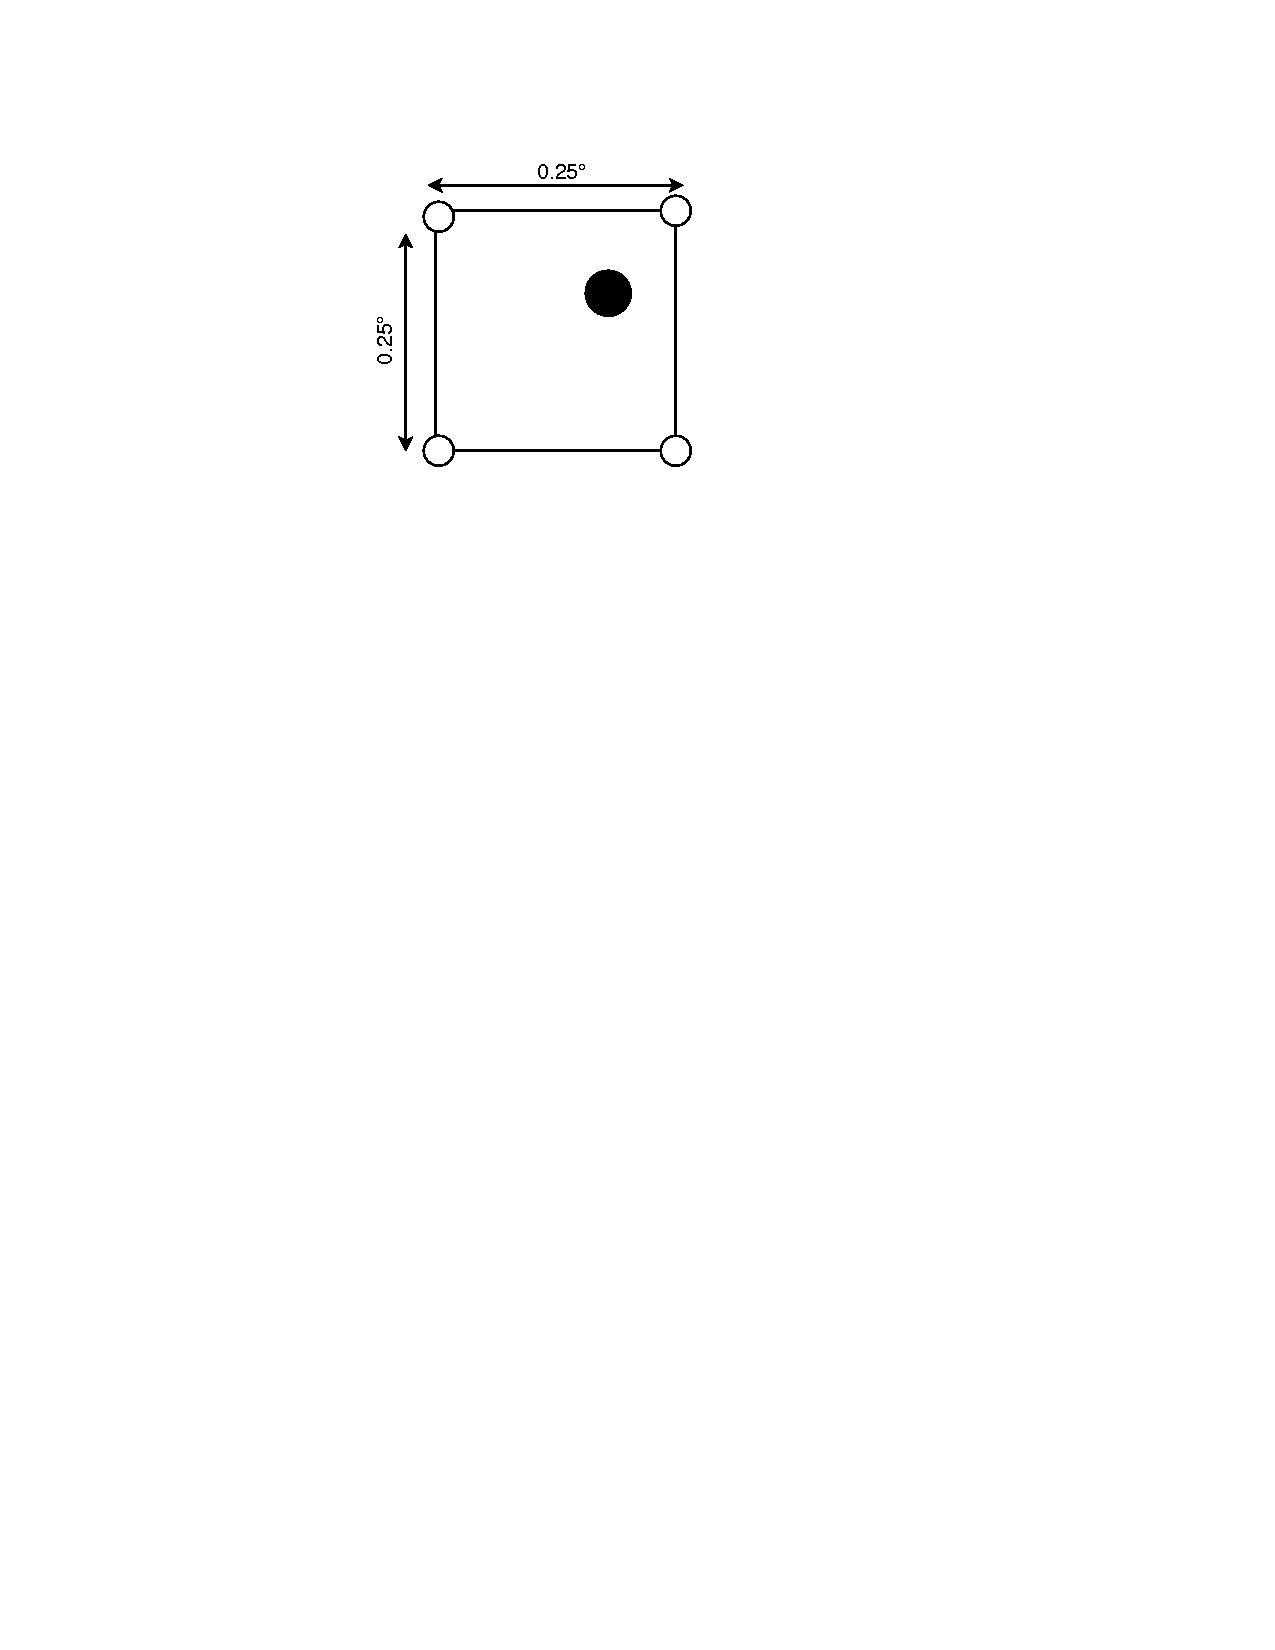
\includegraphics[width=12pc]{figs/point.pdf}
\caption{Acquiring the large-scale predictors by averaging the ERA Interim grid points. The solid circle 
is the location of a point in an MCS trajectory. The four open circles are the ERA Interim grid points, 
which surround the MCS point. The large-scale predictors are computed by averaging these four points.}
\label{figone}
\end{figure}

\begin{figure}[h] %Fig2
\centering
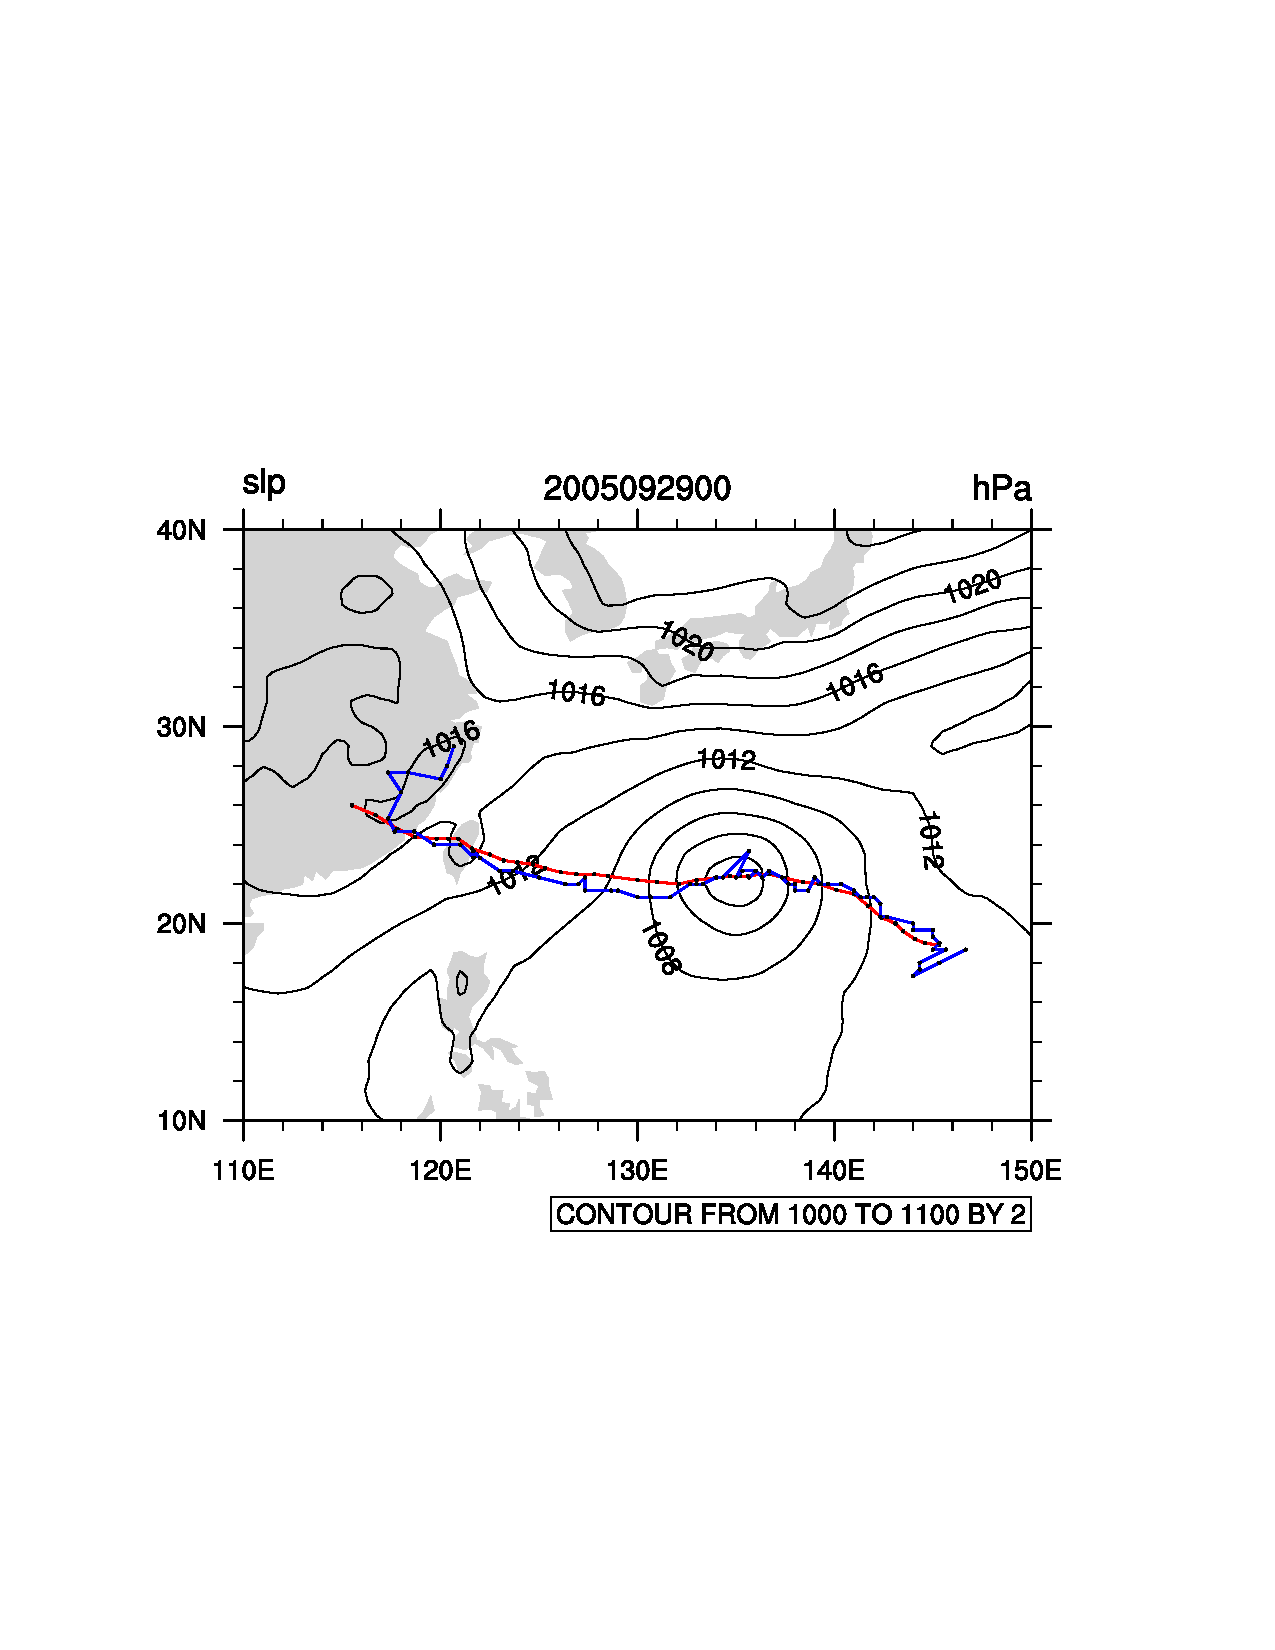
\includegraphics[width=30pc]{figs/obs_validation.pdf}
\caption{ERA Interim sea level pressure. ERA-Interim sea level pressure. Red line is the trajectory of TC. 
Blue line is the trajectory of MCS.}
\label{figone}
\end{figure}

\begin{figure}[h] %Fig3
\centering
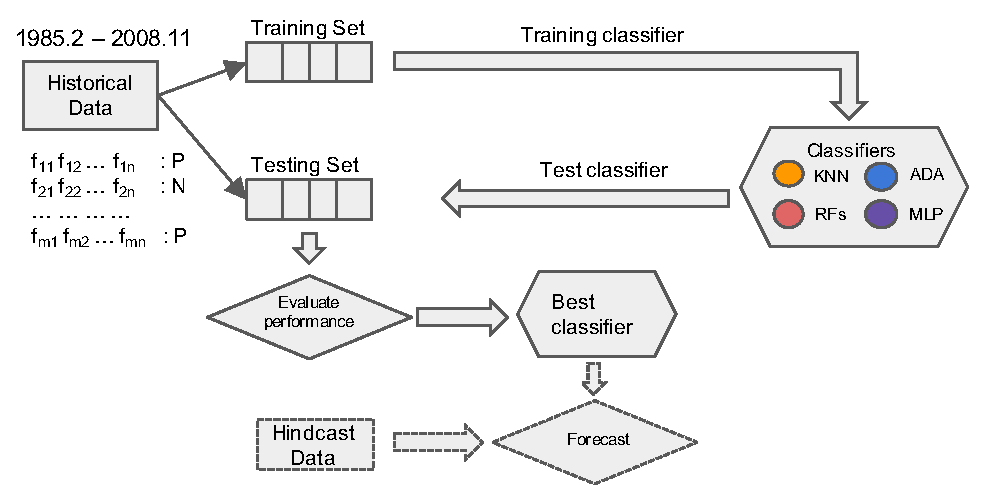
\includegraphics[width=30pc]{figs/workflow.pdf}
\caption{Flow diagram of TC genesis prediction using machine learning.}
\label{figone}
\end{figure}

\begin{figure}[h] %Fig4
\centering
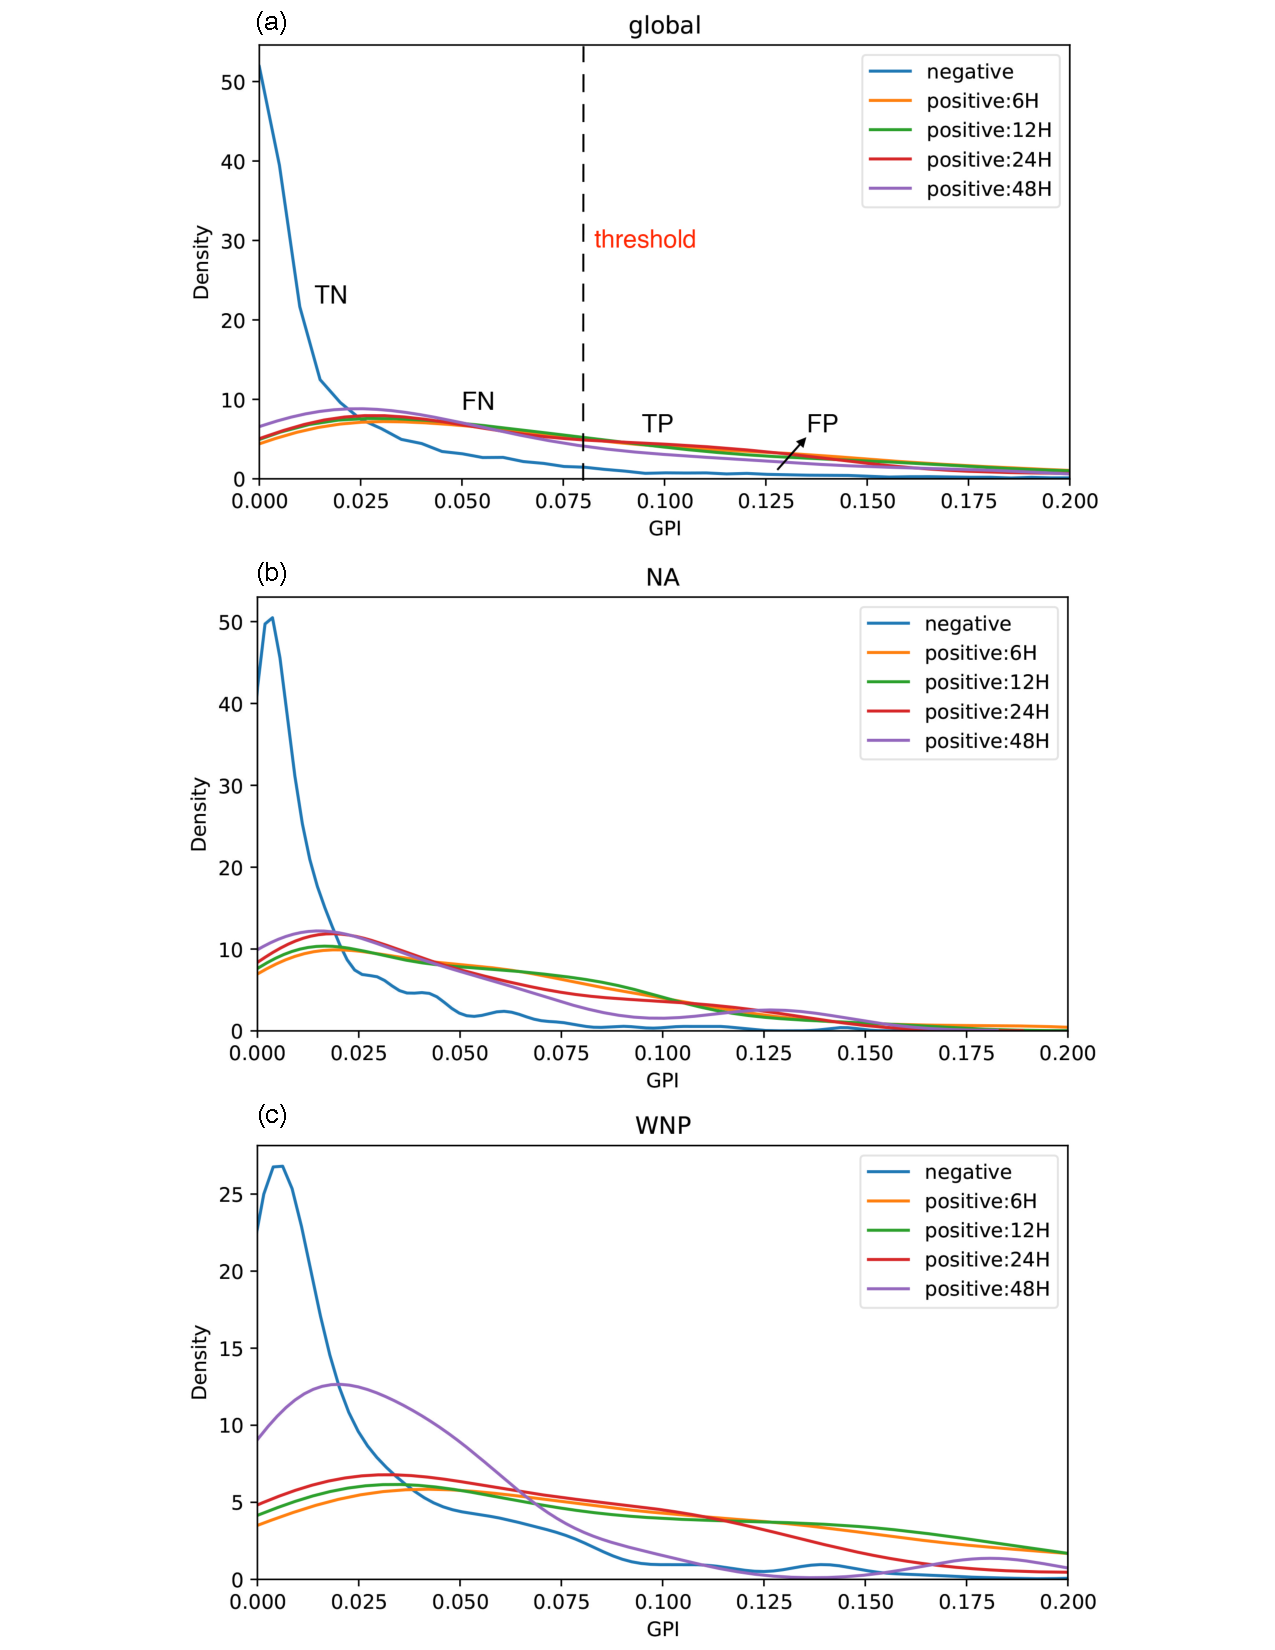
\includegraphics[width=20pc]{figs/kde.pdf}
%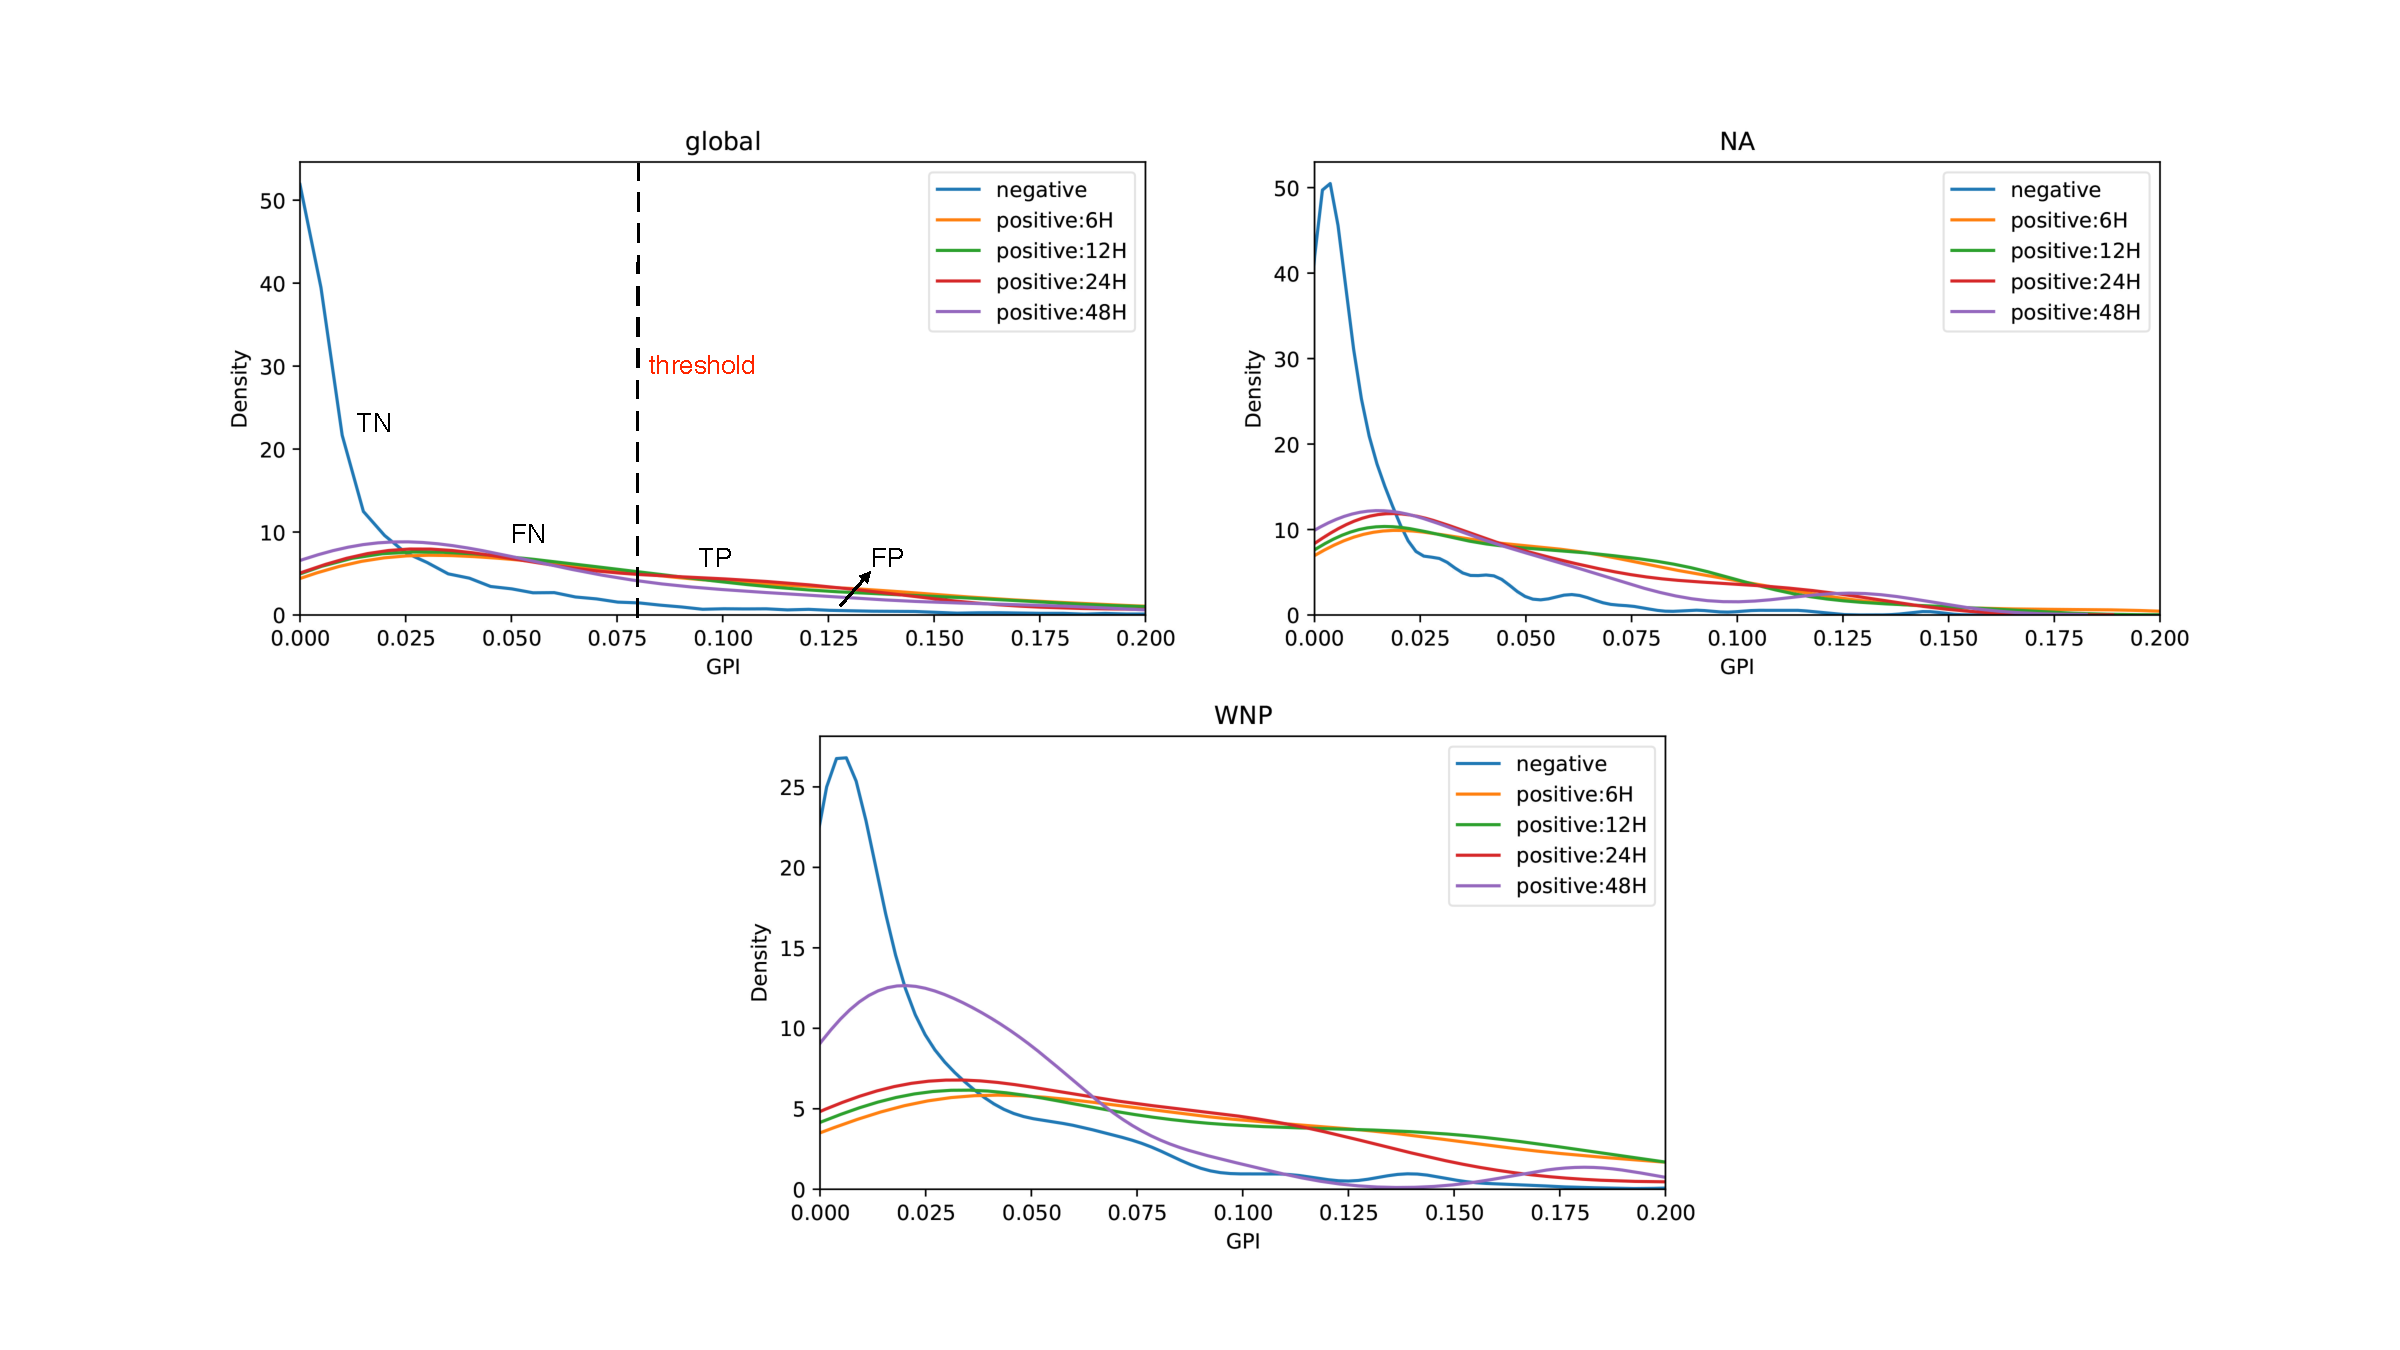
\includegraphics[width=40pc]{figs/kde_tight.pdf}
\caption{The GPI KDE of negative case and positive cases under various lead times. }
\label{figone}
\end{figure}

%\begin{figure}[h] %Fig5
%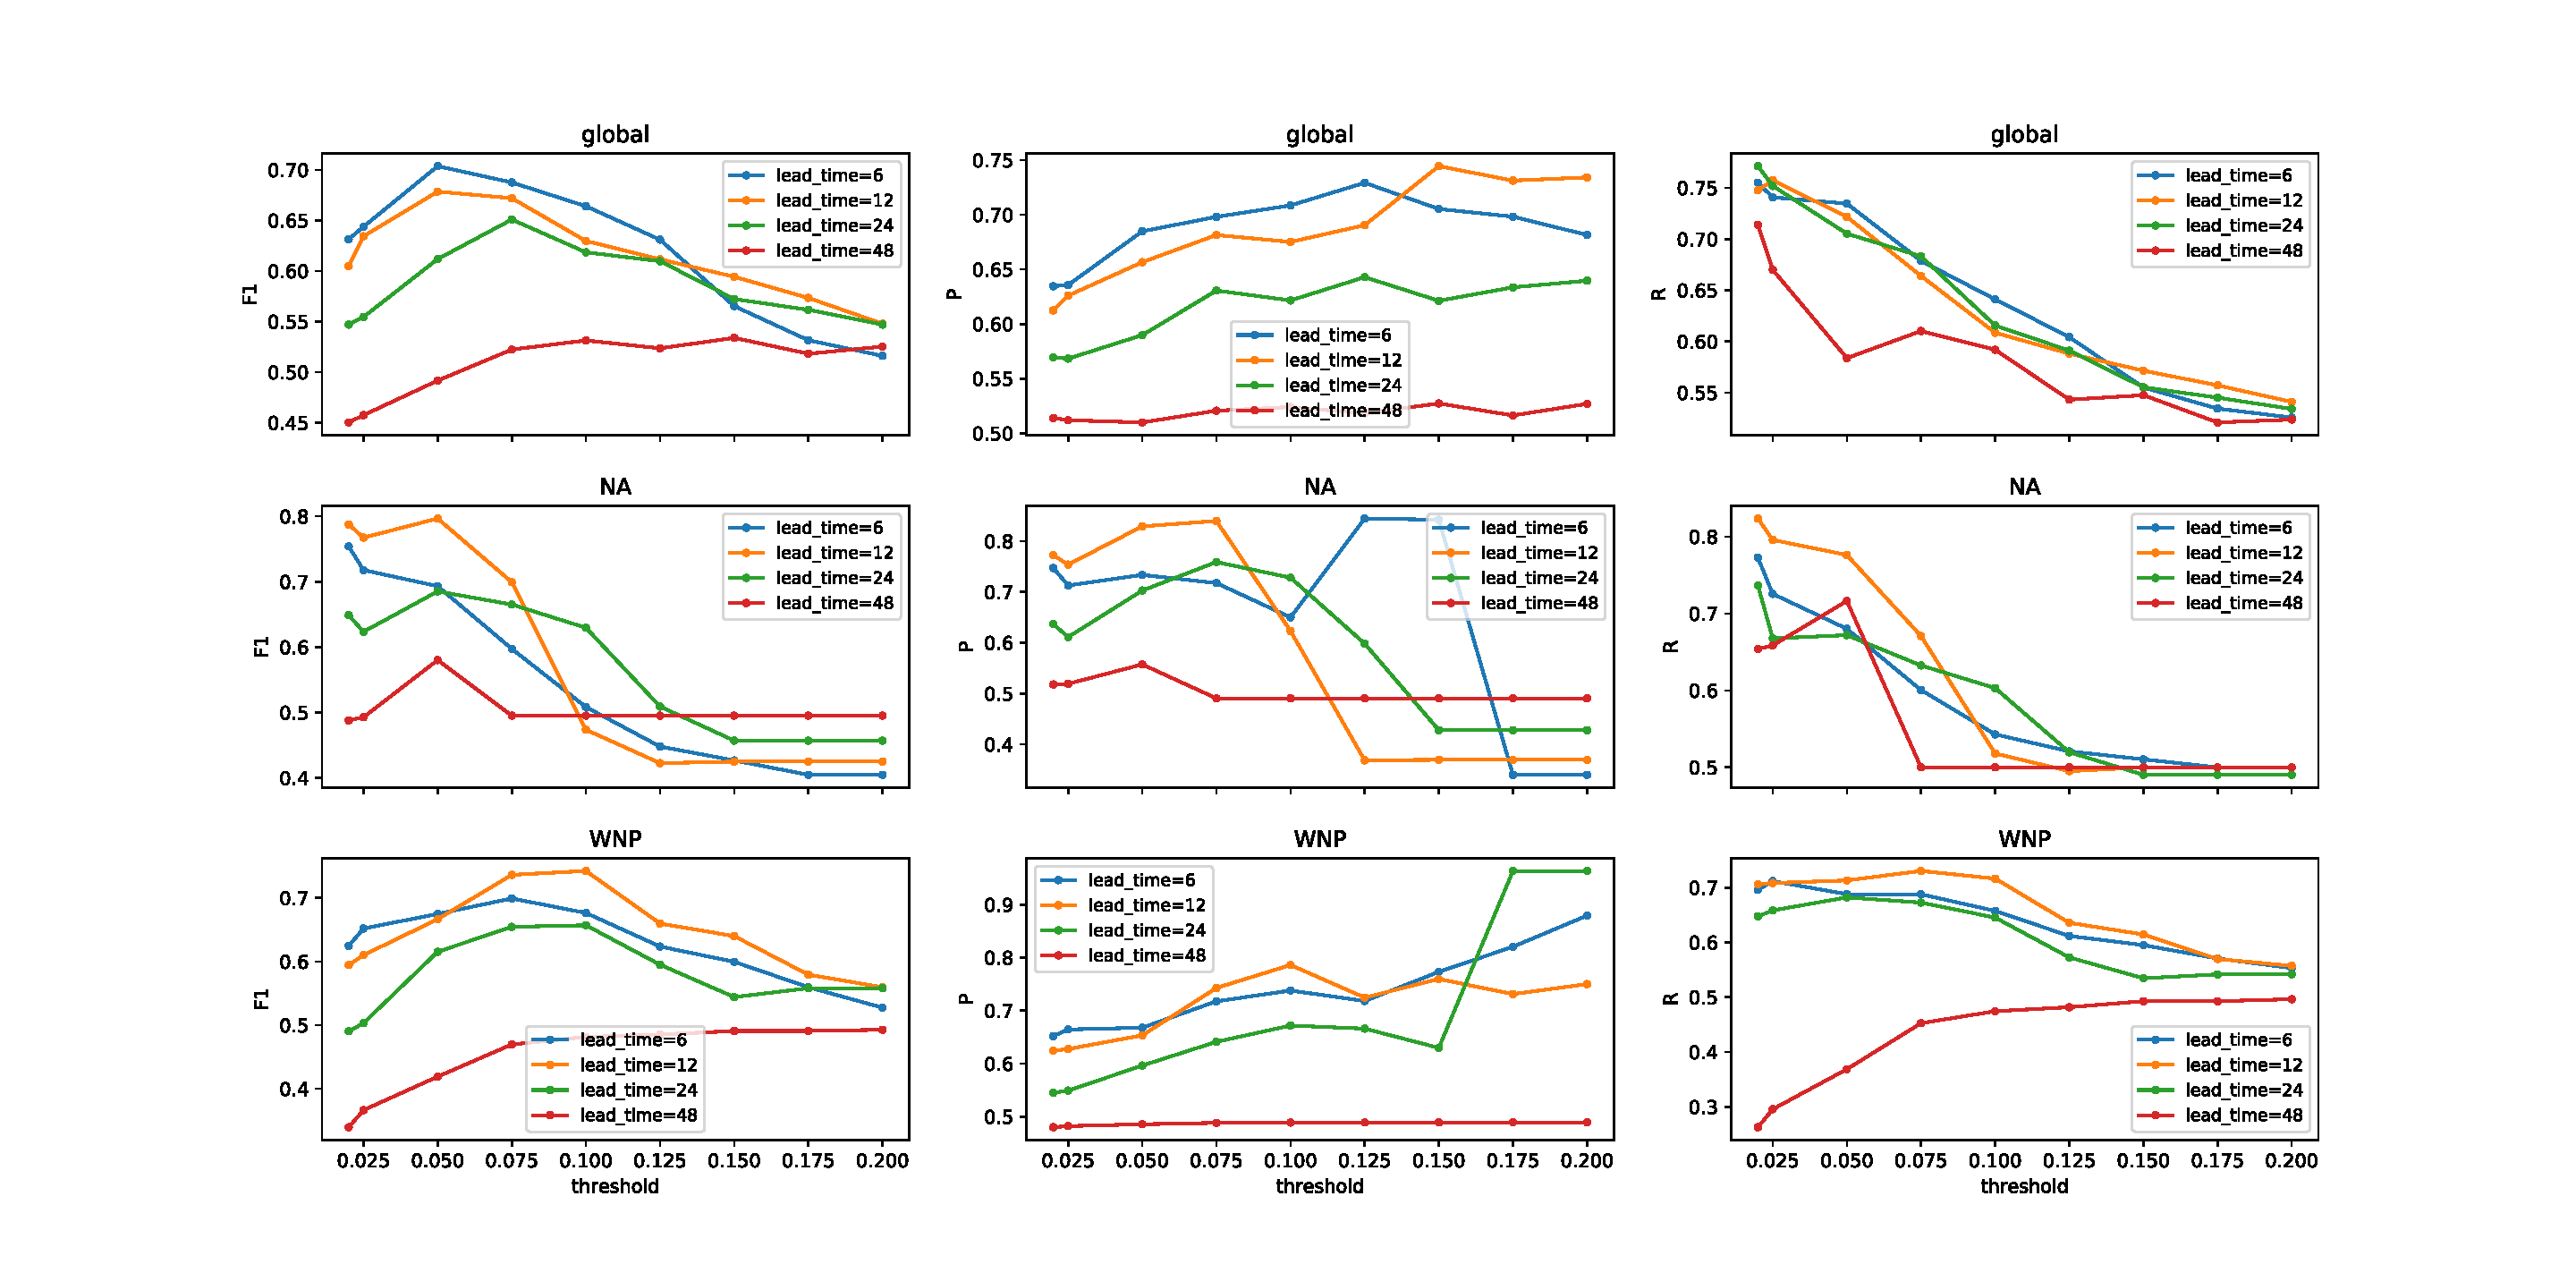
\includegraphics[width=30pc]{figs/GPI_thres.pdf}
%\caption{ }
%\label{figone}
%\end{figure}

\begin{figure}[h] %Fig5
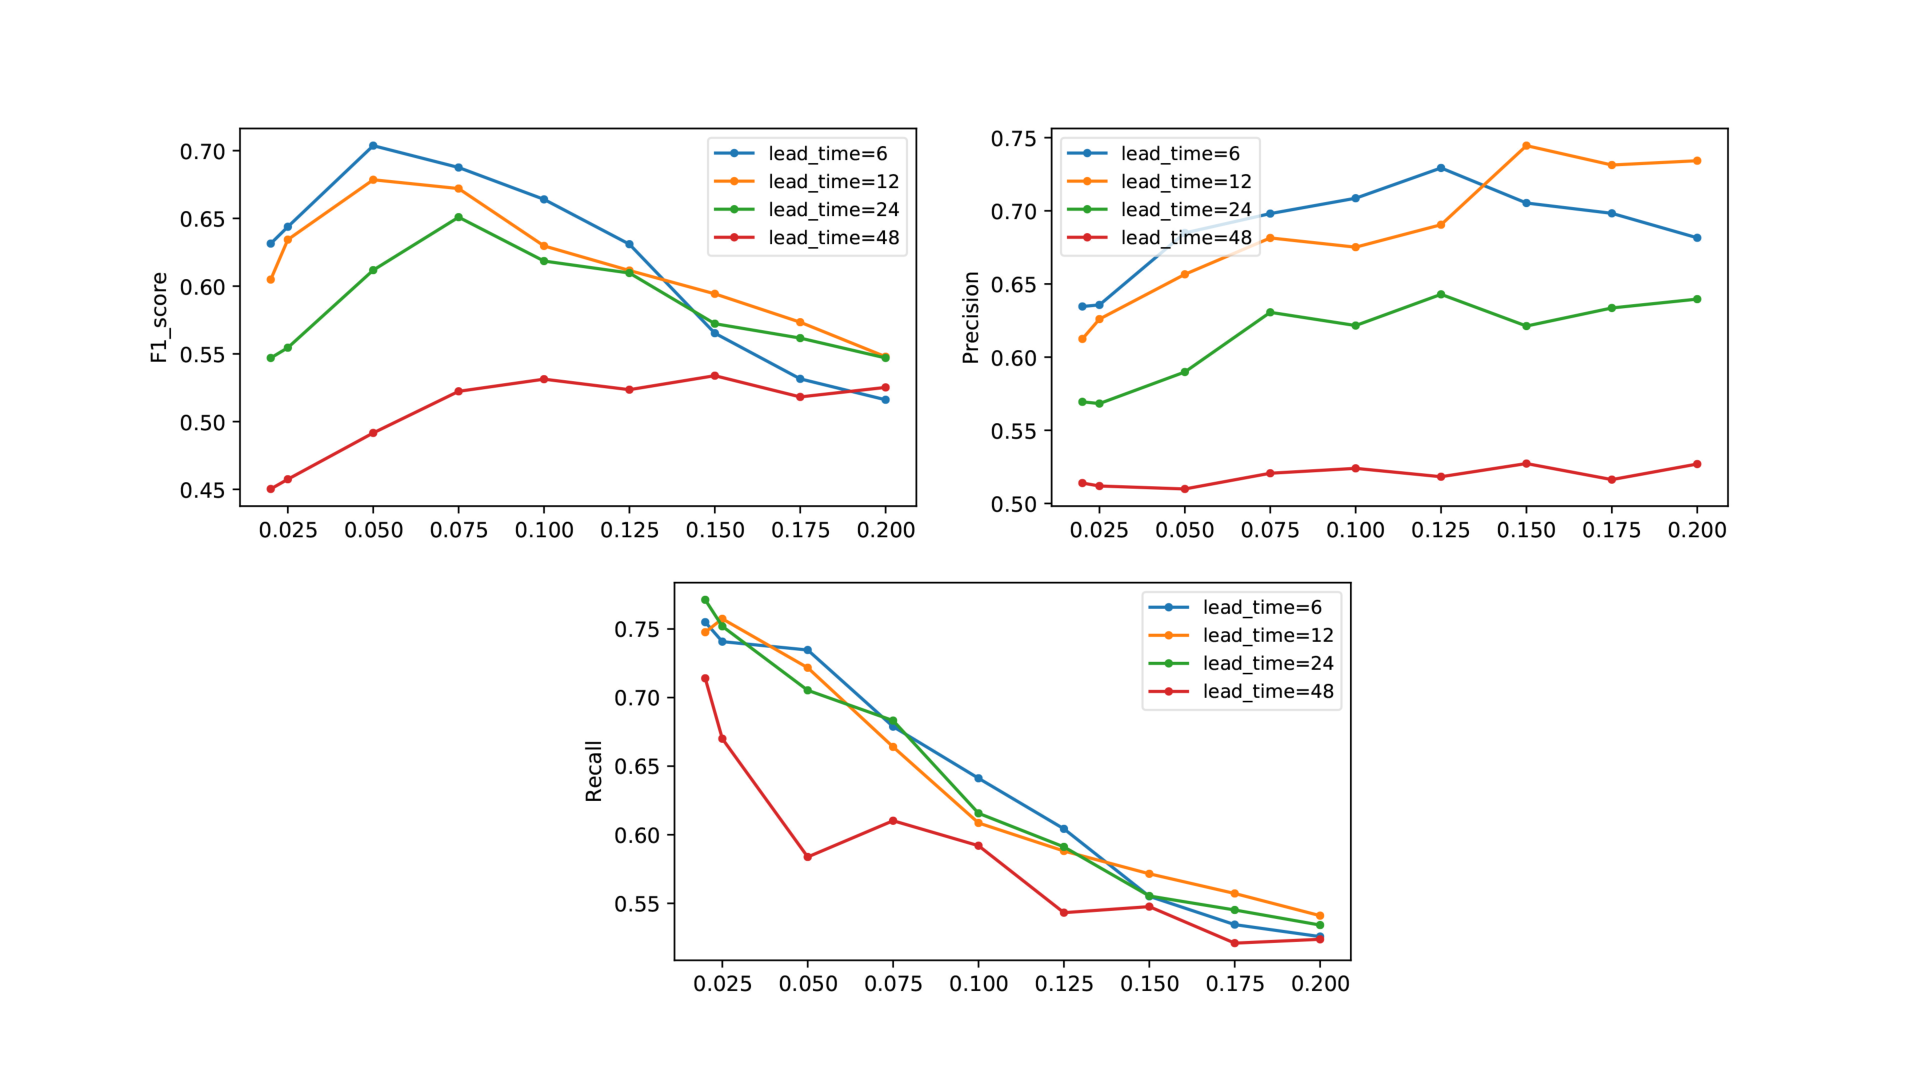
\includegraphics[width=30pc]{figs/GPI_thres_global_f1.pdf}
\caption{Performance of GPI threshold classifier in global tropical.}
\label{figone}
\end{figure}

\begin{figure}[h] %Fig6
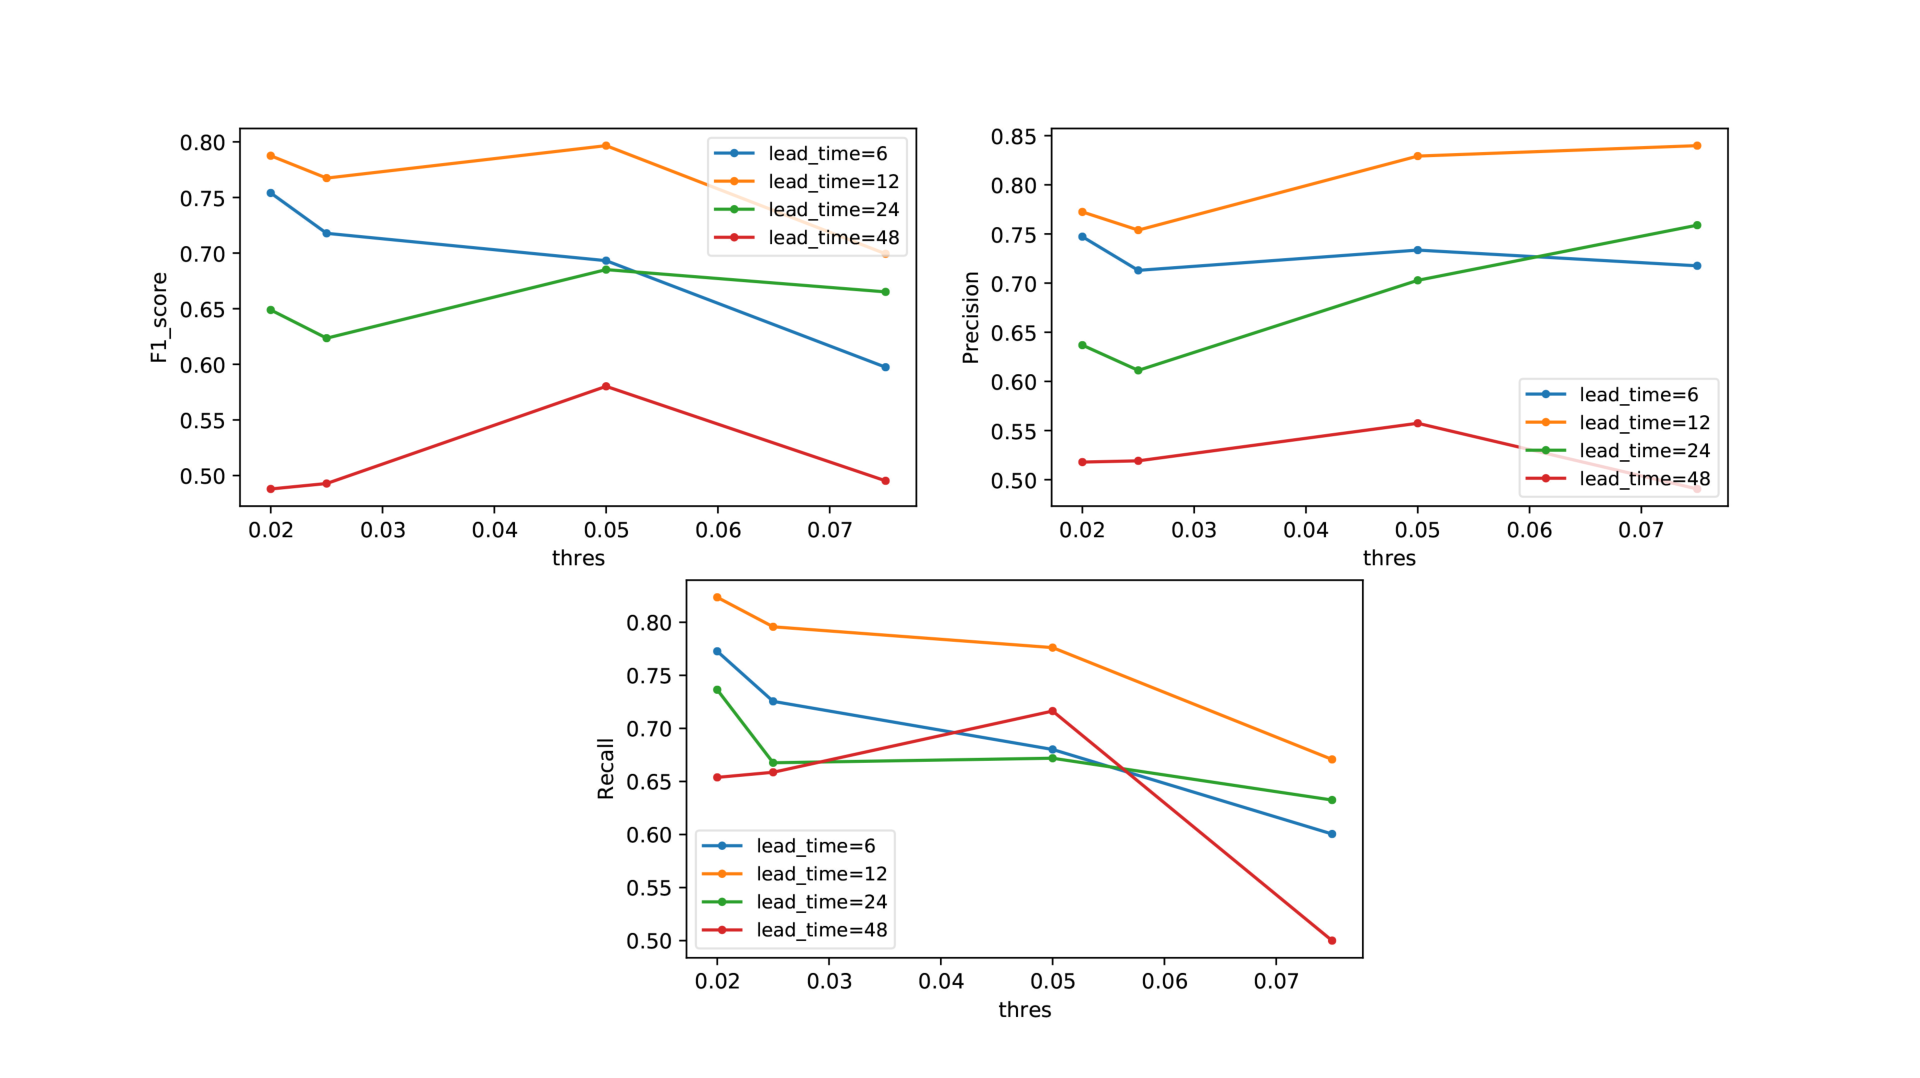
\includegraphics[width=30pc]{figs/GPI_thres_NA_f1.pdf}
\caption{Same as Figure 5, but for North Atlantic Ocean. }
\label{figone}
\end{figure}

\begin{figure}[h] %Fig7
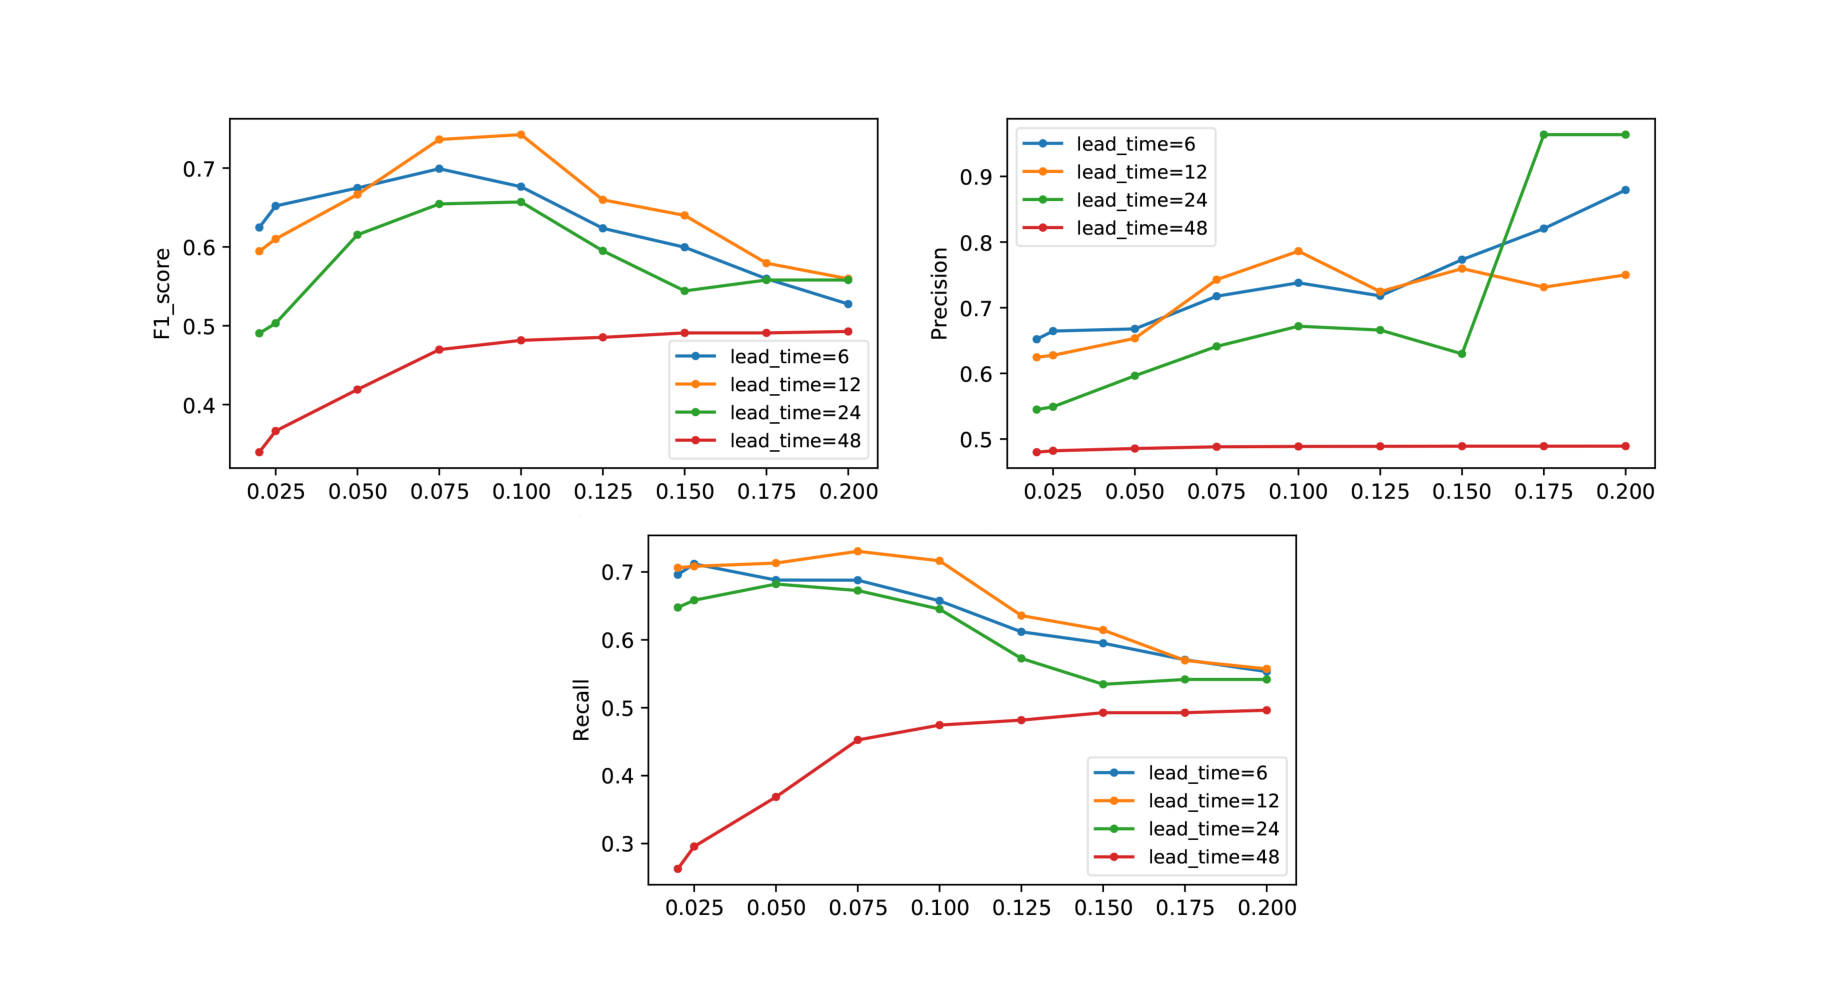
\includegraphics[width=30pc]{figs/GPI_thres_WNP_f1.pdf}
\caption{Same as Figure 5, but for Western East Pacific Ocean.}
\label{figone}    
\end{figure}

\begin{figure}[h] %Fig8
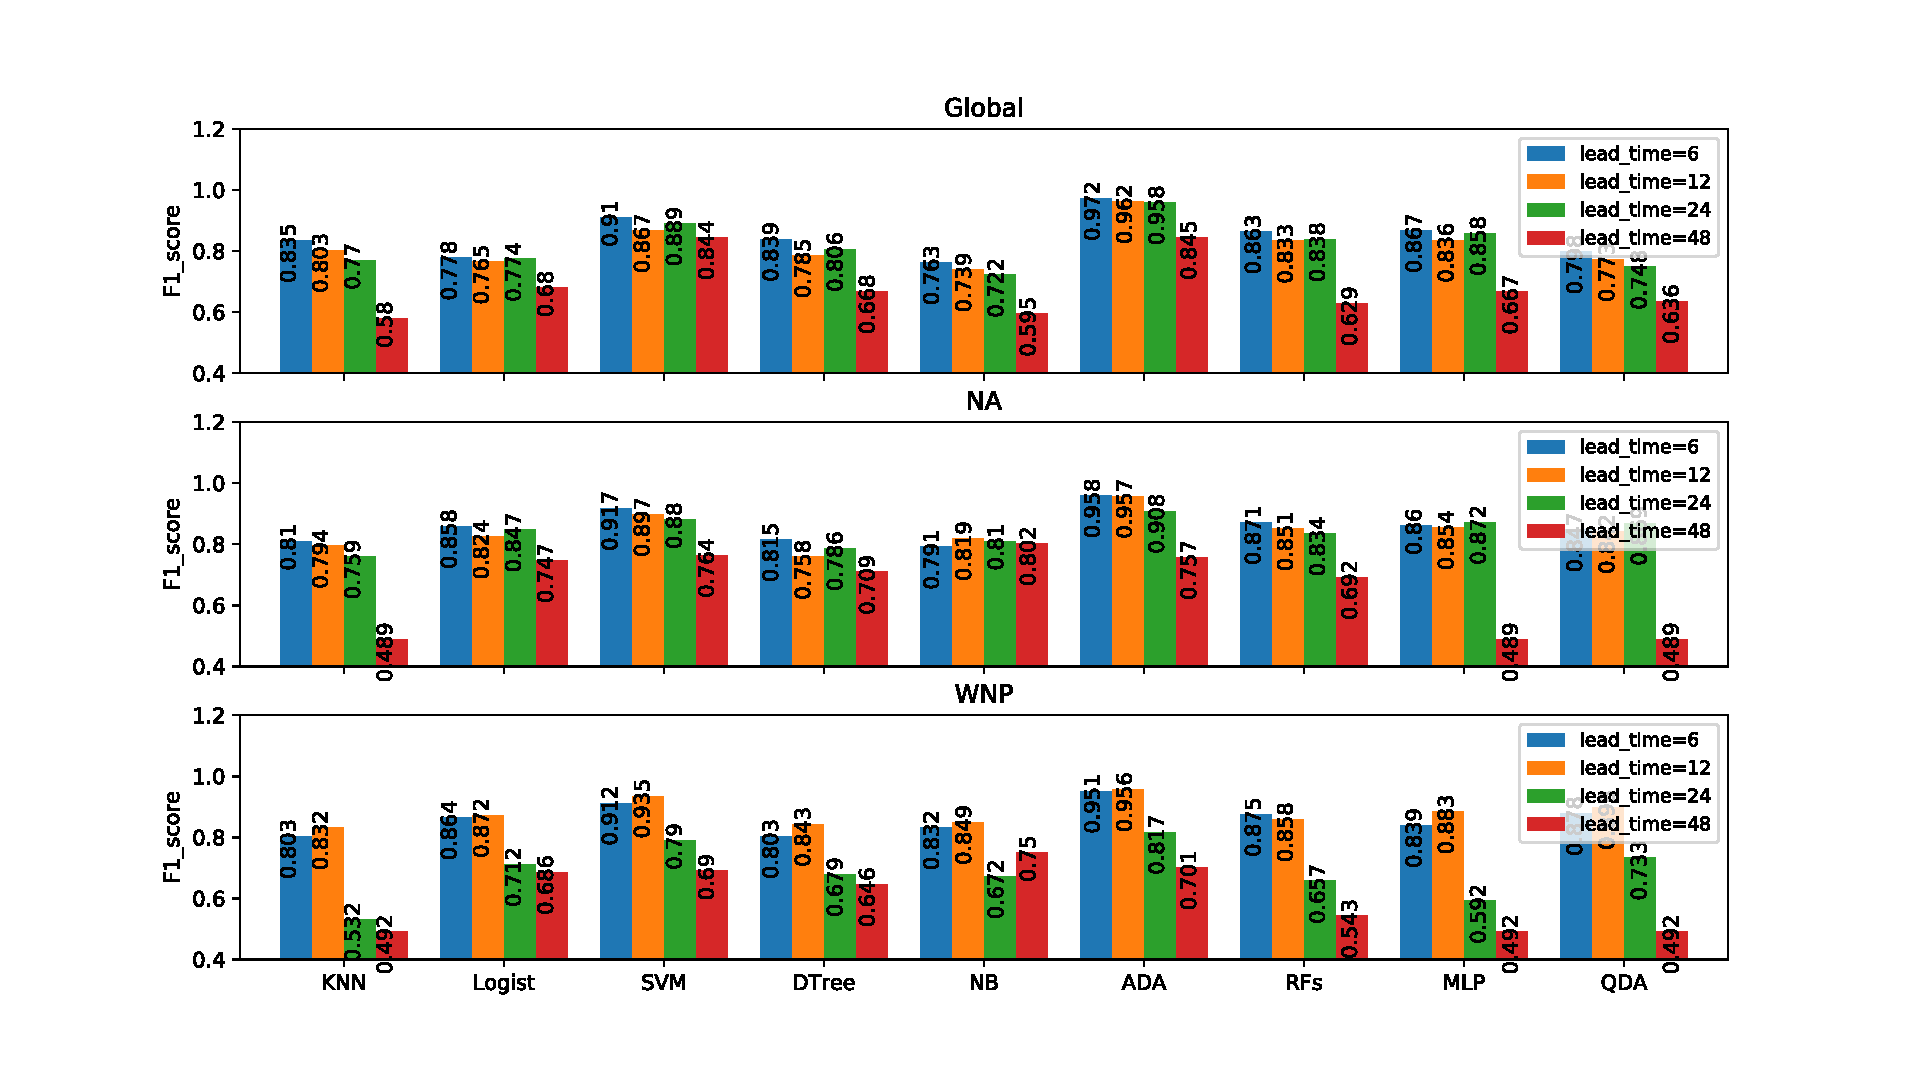
\includegraphics[width=30pc]{figs/alg_F1.pdf}
\caption{The F1 score of machine learning classifiers in global tropical, North Atlantic 
and Western East Pacific Ocean.}
\label{figone}    
\end{figure}

\begin{figure}[h] %Fig9
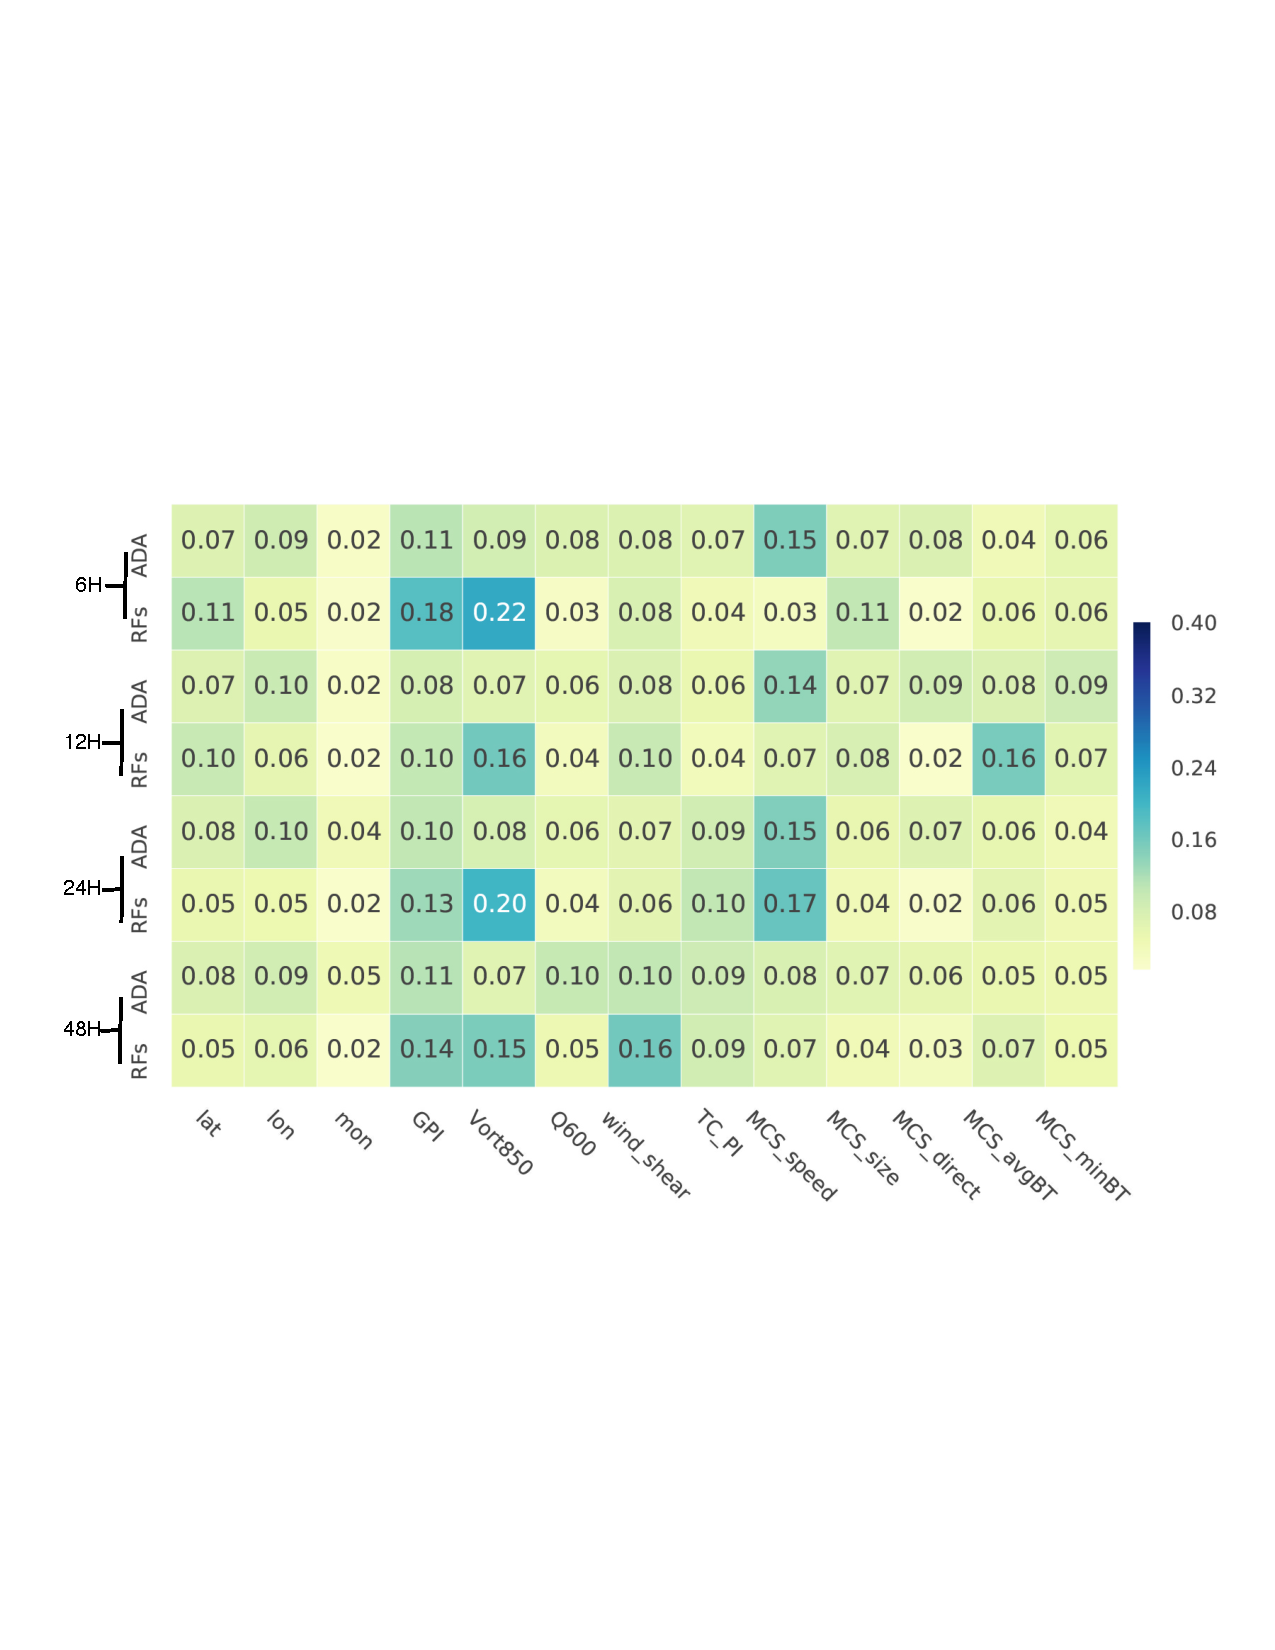
\includegraphics[width=30pc]{figs/imp_global.pdf}
\caption{Factor importance computed by Adaboost and Random Forests under 6\-hour, 12\-hour, 24\-hour and 48\-hour lead times.}
\label{figone}
\end{figure}

\begin{figure}[h] %Fig10
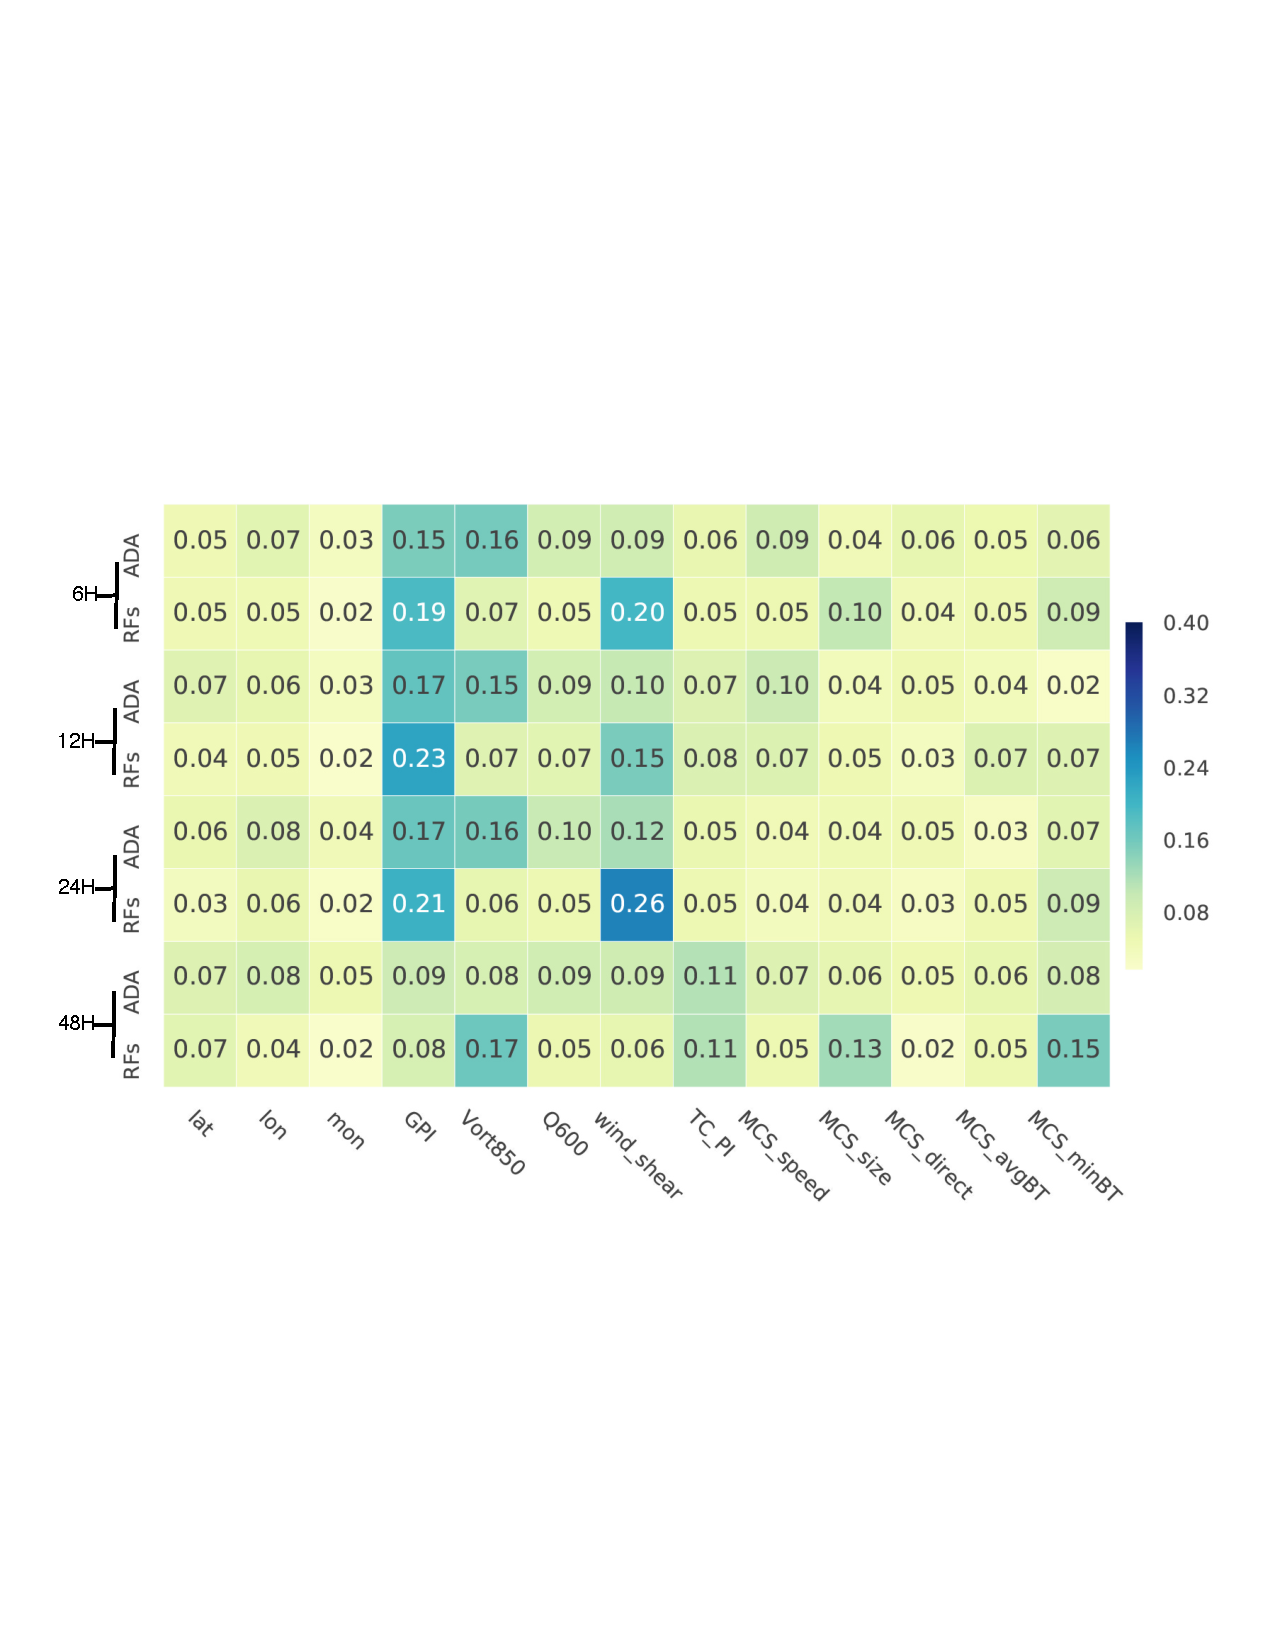
\includegraphics[width=30pc]{figs/imp_NA.pdf}
\caption{Same as Figure 9, but for North Atlantic Ocean.}
\label{figone}
\end{figure}

\begin{figure}[h] %Fig11
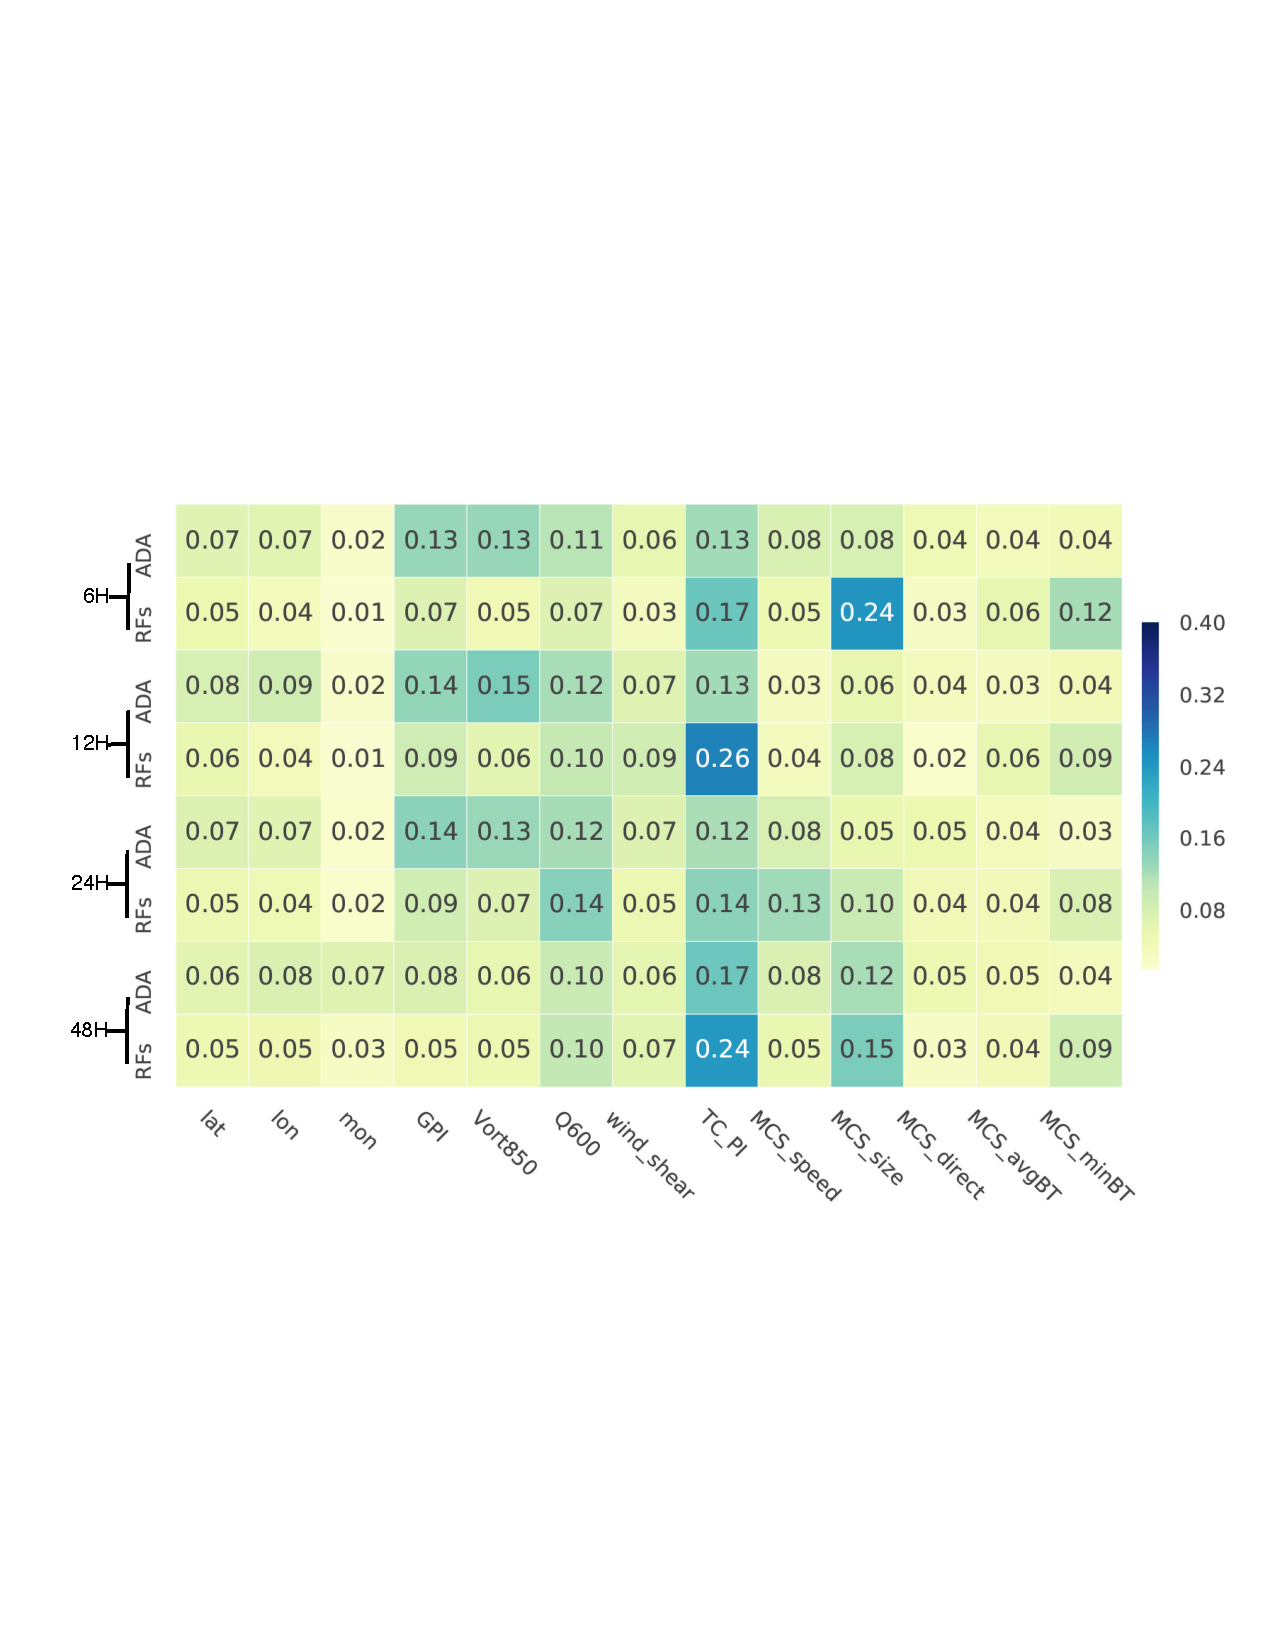
\includegraphics[width=30pc]{figs/imp_WNP.pdf}
\caption{Same as Figure 9, but for Western East Pacific Ocean.}
\label{figone}
\end{figure}

\end{document}